%% 12min talk

\documentclass[english]{beamer}
\usetheme{Warsaw}
\setbeamertemplate{navigation symbols}{} % remove the navigation symbols
\setbeamertemplate{headline}{} % remove headline
\setbeamertemplate{footline}[frame number]

\usepackage{babel}
\usepackage[utf8]{inputenc}
\usepackage{textcomp}
\usepackage{wasysym}
\usepackage{diagmac2}
\usepackage{cancel}
\usepackage{xcolor}

\title{Variational Bayes Applied to Multimodal Distributions in B Physics}
\author{S.~Jahn\inst{1} \and F.~Beaujean\inst{2} \and C.~Bobeth\inst{3}}
\institute{
    \inst{1}
    Exzellenzcluster Universe\\
    Technische Universität München
    \and
    \inst{2}
    Exzellenzcluster Universe\\
    Ludwig-Maximilians-Universität München
    \and
    \inst{3}
    Institute for Advanced Study\\
    Technische Universität München
}
\date{March 12\\DPG Wuppertal 2015}

% ----------------------------------------------------------------------

\newcommand{\slide}[2][t]{\begin{frame}[#1] \frametitle{\insertsubsectionhead} #2 \end{frame}}
\newcommand{\KLPp}[0]{KL( P\|{}p)}
\newcommand{\KLqp}[0]{KL( q\|{}p)}
\newcommand{\varmuN}{var(\mu^{N})}
\newcommand{\wilsoncten }{\mathcal{C} ^{      } _{10}}
\newcommand{\wilsonctenp}{\mathcal{C} ^{\prime} _{10}}
\newcommand{\errorasymm}[3]{#1 \substack{\hspace{.05em} \scriptscriptstyle + \hspace{.05em} #2 \\ \scriptscriptstyle -#3} } % asymmetric uncertainties
\newcommand{\gauss}{\mathcal{N}}
\newcommand{\rmdx}[1]{\mbox{d} #1 \,} % differential d
\newcommand{\samples}{\boldsymbol{X}}
\newcommand{\red}[1]{\textcolor{red}{#1}}

\renewcommand\CancelColor{\color{red}}

\setbeamercolor{block title}{bg=blue, fg=white}

\begin{document}

% ----------------------- title page, unnumbered -----------------------

{
\setbeamertemplate{footline}{}
\frame[nopagenumbering,noframenumbering]{\titlepage}
}
% ------------------------- B-physics section --------------------------

\section{Scalar and tensor contributions to $ b \to s \mu^+ \mu^- $}

% TOC-page --> do not show in a 12min talk
% \begin{frame} \frametitle{\insertsectionhead} \tableofcontents[currentsection] \end{frame}

\subsection{Effective theory}

\newcommand{\redsecond}[1]{\uncover<2->{\textcolor{red}{#1}}}

\slide{

    effective Lagrangian for $ b \to s \mu^+ \mu^- $ (\only<1>{$\mathrm{SM}$}\only<2>{\red{beyond}-$\mathrm{SM}$}): \
    \
    \newline \newline \

    $$ \mathcal{L}_{int} = \frac{4 G_F}{\sqrt{2}} \frac{\alpha_e}{4\pi} V_{tb}^{} V_{ts}^\ast \sum_i \mathcal{C}_i \mathcal{O}_i + ... + \text{h.c.} $$

    ~ \newline

    \begin{center}
      \begin{tabular}{cc}
          \small $ \mathcal{O}_{9} ^{\redsecond{(\prime)}} = \left[\bar{s} \gamma_\mu^{} P_{L\redsecond{(R)}} b\right]\!\left[\bar{\ell} \gamma^\mu \ell\right] $
                & \small $  \mathcal{O}_{10}^{\redsecond{(\prime)}} = \left[\bar{s} \gamma_\mu^{} P_{L\redsecond{(R)}} b\right]\!\left[\bar{\ell} \gamma^\mu \gamma_5 \ell\right] $ \\[1cm]
          \Large $ \begin{aligned}
                \redsecond{\mathcal{O}_S^{(\prime)}}    & \redsecond{= \left[\bar{s} P_{R\redsecond{(L)}} b\right]\!\left[\bar{\ell} \ell\right]} \\[5mm]
                \redsecond{\mathcal{O}_T}               & \redsecond{= \left[\bar{s} \sigma_{\mu\nu}^{} b\right]\!\left[\bar{\ell} \sigma^{\mu\nu} \ell\right] }
          \end{aligned} $ & \Large $ \begin{aligned}
                \redsecond{\mathcal{O}_P^{(\prime)}}    & \redsecond{= \left[\bar{s} P_{R(L)} b\right]\!\left[\bar{\ell} \gamma_5 \ell\right] } \\[5mm]
                \redsecond{\mathcal{O}_{T5}}            & \redsecond{= \left[\bar{s} \sigma_{\mu\nu}^{} b\right]\!\left[\bar{\ell} \sigma^{\mu\nu} \gamma_5 \ell\right] }
          \end{aligned} $
     \end{tabular}
    \end{center}

}

\subsection{Sensitive observables}
\newcommand{\sqrtqsq}{\sqrt{q^2}}

\slide{

    \begin{itemize}

        \item {\large\textbf{$\boldsymbol{B\rightarrow K\mu^+\mu^-}$ angular distribution} }

        \uncover<2->{$$
            \frac{1}{\Gamma} \frac{\mbox{d}\Gamma}{\mbox{d}\!\cos\theta}
            = \frac{3}{4} (1 - \red{F_H}) \sin^2\!\theta
            + \frac{1}{2} \red{F_H}
            + \red{A_{FB}} \cos\theta
        $$}

        \begin{align*}
            \uncover<3->{\red{A_{FB}} \propto &
            \mbox{Re}\big[(\mathcal{C}_{P} + \mathcal{C}_{P} ^\prime)\, \mathcal{C}_{T5} ^\ast
                        + (\mathcal{C}_{S} + \mathcal{C}_{S} ^\prime)\, \mathcal{C}_{T}  ^\ast
                        + \mathcal{O}(m_\ell/\sqrtqsq)\big] \Big/ \Gamma}
            \\
            \uncover<4->{\red{F_H} \propto & \Big[
              \ldots \left(|\mathcal{C}_{T}|^2 + |\mathcal{C}_{T5}|^2\right)
             + \ldots \left(|\mathcal{C}_{S} + \mathcal{C}_{S} ^\prime)|^2 + |\mathcal{C}_{P} + \mathcal{C}_{P} ^\prime|^2 \right) \\
             & + \mathcal{O}(m_\ell/\sqrtqsq)
            \Big] \Big/ \Gamma} \\
        \end{align*}

        \vspace{-9mm}

        \uncover<5->{$$ F_{H}^\mathrm{SM} = \mathcal{O}(m_\ell ^2/ q^2) ~~~~~ A_{FB}^\mathrm{SM} = 0 $$}

        \item {\large\textbf{$\boldsymbol{B_s\rightarrow \mu^+\mu^-}$ branching fraction} }

        \vspace{-4mm}

        \uncover<6->{\begin{align*}
            \red{\mathcal{B}(B_s\rightarrow\mu^+\mu^-)} \propto | \mathcal{C}_{S} - \mathcal{C}_{S} ^\prime |^2 +
            |( \mathcal{C}_{P} - \mathcal{C}_{P} ^\prime ) + \frac{2 m_\ell}{M_{B_s}}( \wilsoncten - \wilsonctenp ) |^2
        \end{align*}}

    \end{itemize}

}

\subsection{Methodology}

\slide{

    we want:
    \newline
    $$ P(\boldsymbol{\theta} | \mathcal{D}, \mathrm{M} ) \overset{\mathrm{Bayes}}{\propto} P(\mathcal{D}|\boldsymbol{\theta}, \mathrm{M})P(\boldsymbol{\theta} | \mathrm{M}) $$

    \only<2->{

        \vspace{1.6mm}

        split theory and experiment - \emph{observables} $\boldsymbol{O}$:

        \only<-5|handout:0>{$$ P(\mathcal{D}|\boldsymbol{\theta}, \mathrm{M})
          = P(\mathcal{D} | \boldsymbol{O} (\boldsymbol{\theta} , \mathrm{M} )) $$}

        \only<6->{$$ P(\mathcal{D}|\boldsymbol{\theta}, \mathrm{M})
          = P(\mathcal{D} | \boldsymbol{O} (\boldsymbol{\theta} , \mathrm{M} ) , \underset{ \text{\textcolor{red}{\textbf{assumption} }} } {\cancel{\boldsymbol{\textcolor{red}{\theta , \mathrm{M}}}}} ) $$}

        \vspace{-6.5mm}

        \only<3->{

            \begin{center}
                \begin{columns}[t] % the "t" option specifies top vertical alignment

                    \column{.5\textwidth}
                        \begin{block}{\center theory}
                            \begin{center}
                                \only<-3|handout:0>{ ~ \vspace{8.4mm} ~ }
                                \only<4->{~~~\emph{calculate} observables \newline
                                $ \boldsymbol{O}(\boldsymbol{\theta} , \mathrm{M}) $}
                            \end{center}
                        \end{block}
                        \only<4->{\center 
\includegraphics[height=1.5cm]{figures/theorist}}

                    \column{.5\textwidth}
                        \begin{block}{\center experiment}
                            \begin{center}
                                \only<-4|handout:0>{ ~ \vspace{8.4mm} ~ }
                                \only<5->{~~~~~\emph{measure} observables \newline
                                    \only<-5|handout:0>{$P\left(\mathcal{D} | \boldsymbol{O} \right)$}
                                    \only<6->{$P\left(\mathcal{D} | \boldsymbol{O} , \cancel{ \textcolor{red}{\boldsymbol{\theta} , \mathrm{M} } } \right)$ }}
                            \end{center}
                        \end{block}
                        \only<5->{\center 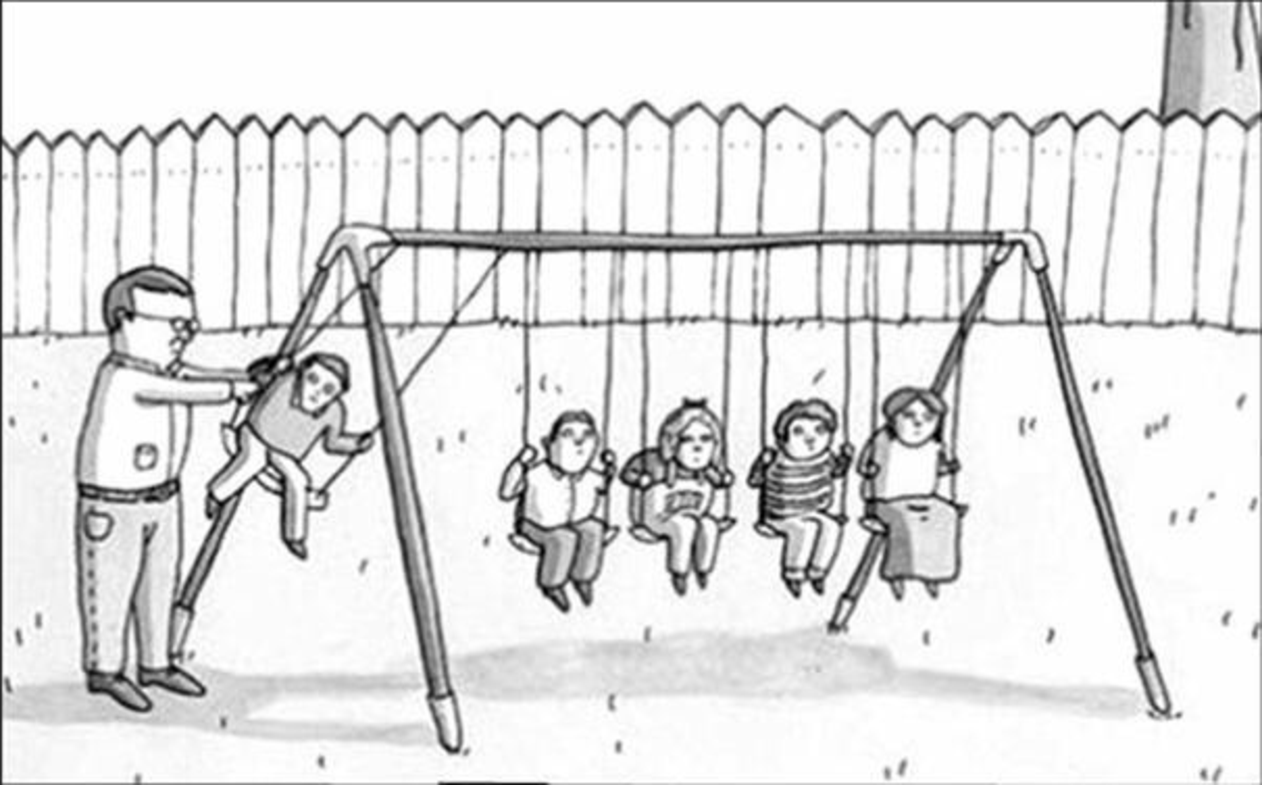
\includegraphics[height=1.5cm]{figures/experimentalist}}

                \end{columns}
            \end{center}
        }

    }

}

\subsection{Measurements $ P\left(\mathcal{D} | \boldsymbol{O} \right) $}

\slide[c]{

    \begin{itemize}
        \item $B\rightarrow K\mu^+\mu^-$: $\mathcal{B} , \red{A_{FB}} , \red{F_H}$
        \begin{itemize}
            \item \red{LHCb 2014 {\tiny (\href{http://arXiv.org/abs/1403.8044}{arXiv:1403.8044} , \href{http://arXiv.org/abs/1403.8045}{arXiv:1403.8045})}}
            \item CDF~ 2012 {\tiny (\url{http://www-cdf.fnal.gov/physics/new/bottom/120628.blessed-b2smumu_96})}
        \end{itemize}

        \item $B_s\rightarrow\mu^+\mu^-$: $\mathcal{B}$

        \begin{itemize}
            \item \red{LHCb+CMS 2014 {\tiny({\href{http://arXiv.org/abs/1411.4413}{arXiv:1411.4413}})}}
        \end{itemize}

        \item $B\rightarrow K^\ast\mu^+\mu^-$: $\mathcal{B}$

        \begin{itemize}
            \item LHCb 2013 {\tiny({\href{http://arXiv.org/abs/1304.6325}{arXiv:1304.6325}})}
            \item CMS~ 2013 {\tiny({\href{http://arXiv.org/abs/1308.3409}{arXiv:1308.3409}})}
            \item CDF~ 2012 {\tiny (\url{http://www-cdf.fnal.gov/physics/new/bottom/120628.blessed-b2smumu_96})}
        \end{itemize}
    \end{itemize}

}

\subsection{Parameters $\boldsymbol{\theta}$}

\slide[c]{

    {\large\textbf{scan parameters}}

    \begin{itemize}
        \item \red{Wilson coefficients $\mathcal{C}_{10} ^{(\prime)} , \mathcal{C}_S ^{(\prime)} , \mathcal{C}_P ^{(\prime)} , \mathcal{C}_T , \text{and} ~ \mathcal{C}_{T5}$}
    \end{itemize}

    \uncover<2->{{\large\textbf{nuisance parameters}}

    \begin{itemize}
        \item CKM matrix (4 parameters)
        \item charm and bottom quark mass (2 parameters)
        \item form factors
              \begin{itemize}
                  \item $B\rightarrow K^{\thinspace\thinspace\thinspace}$ (5 parameters)
                  \item $B\rightarrow K^\ast$                             (6 parameters)
              \end{itemize}
        \item $B_s$ decay constant $f_{B_s}$
        \item subleading corrections (11 parameters)
    \end{itemize}}

    \vspace{5mm}

    \uncover<3->{{\large\textbf{theory calculation $\boldsymbol{O(\theta , M)}$:}}

    \vspace{2.5mm}
    \Large open-source implementation: EOS-package \newline \large \url{http://project.het.physik.tu-dortmund.de/eos/}}

}

\subsection{Joint fit of $\mathcal{C}_{10} ^{(\prime)} , \mathcal{C}_S ^{(\prime)} , \mathcal{C}_P ^{(\prime)} , \mathcal{C}_T , \text{and} ~ \mathcal{C}_{T5}$ }

\slide[c]{

    \vspace{6mm}

    \begin{columns}[c]
        \column{0.65\textwidth}
            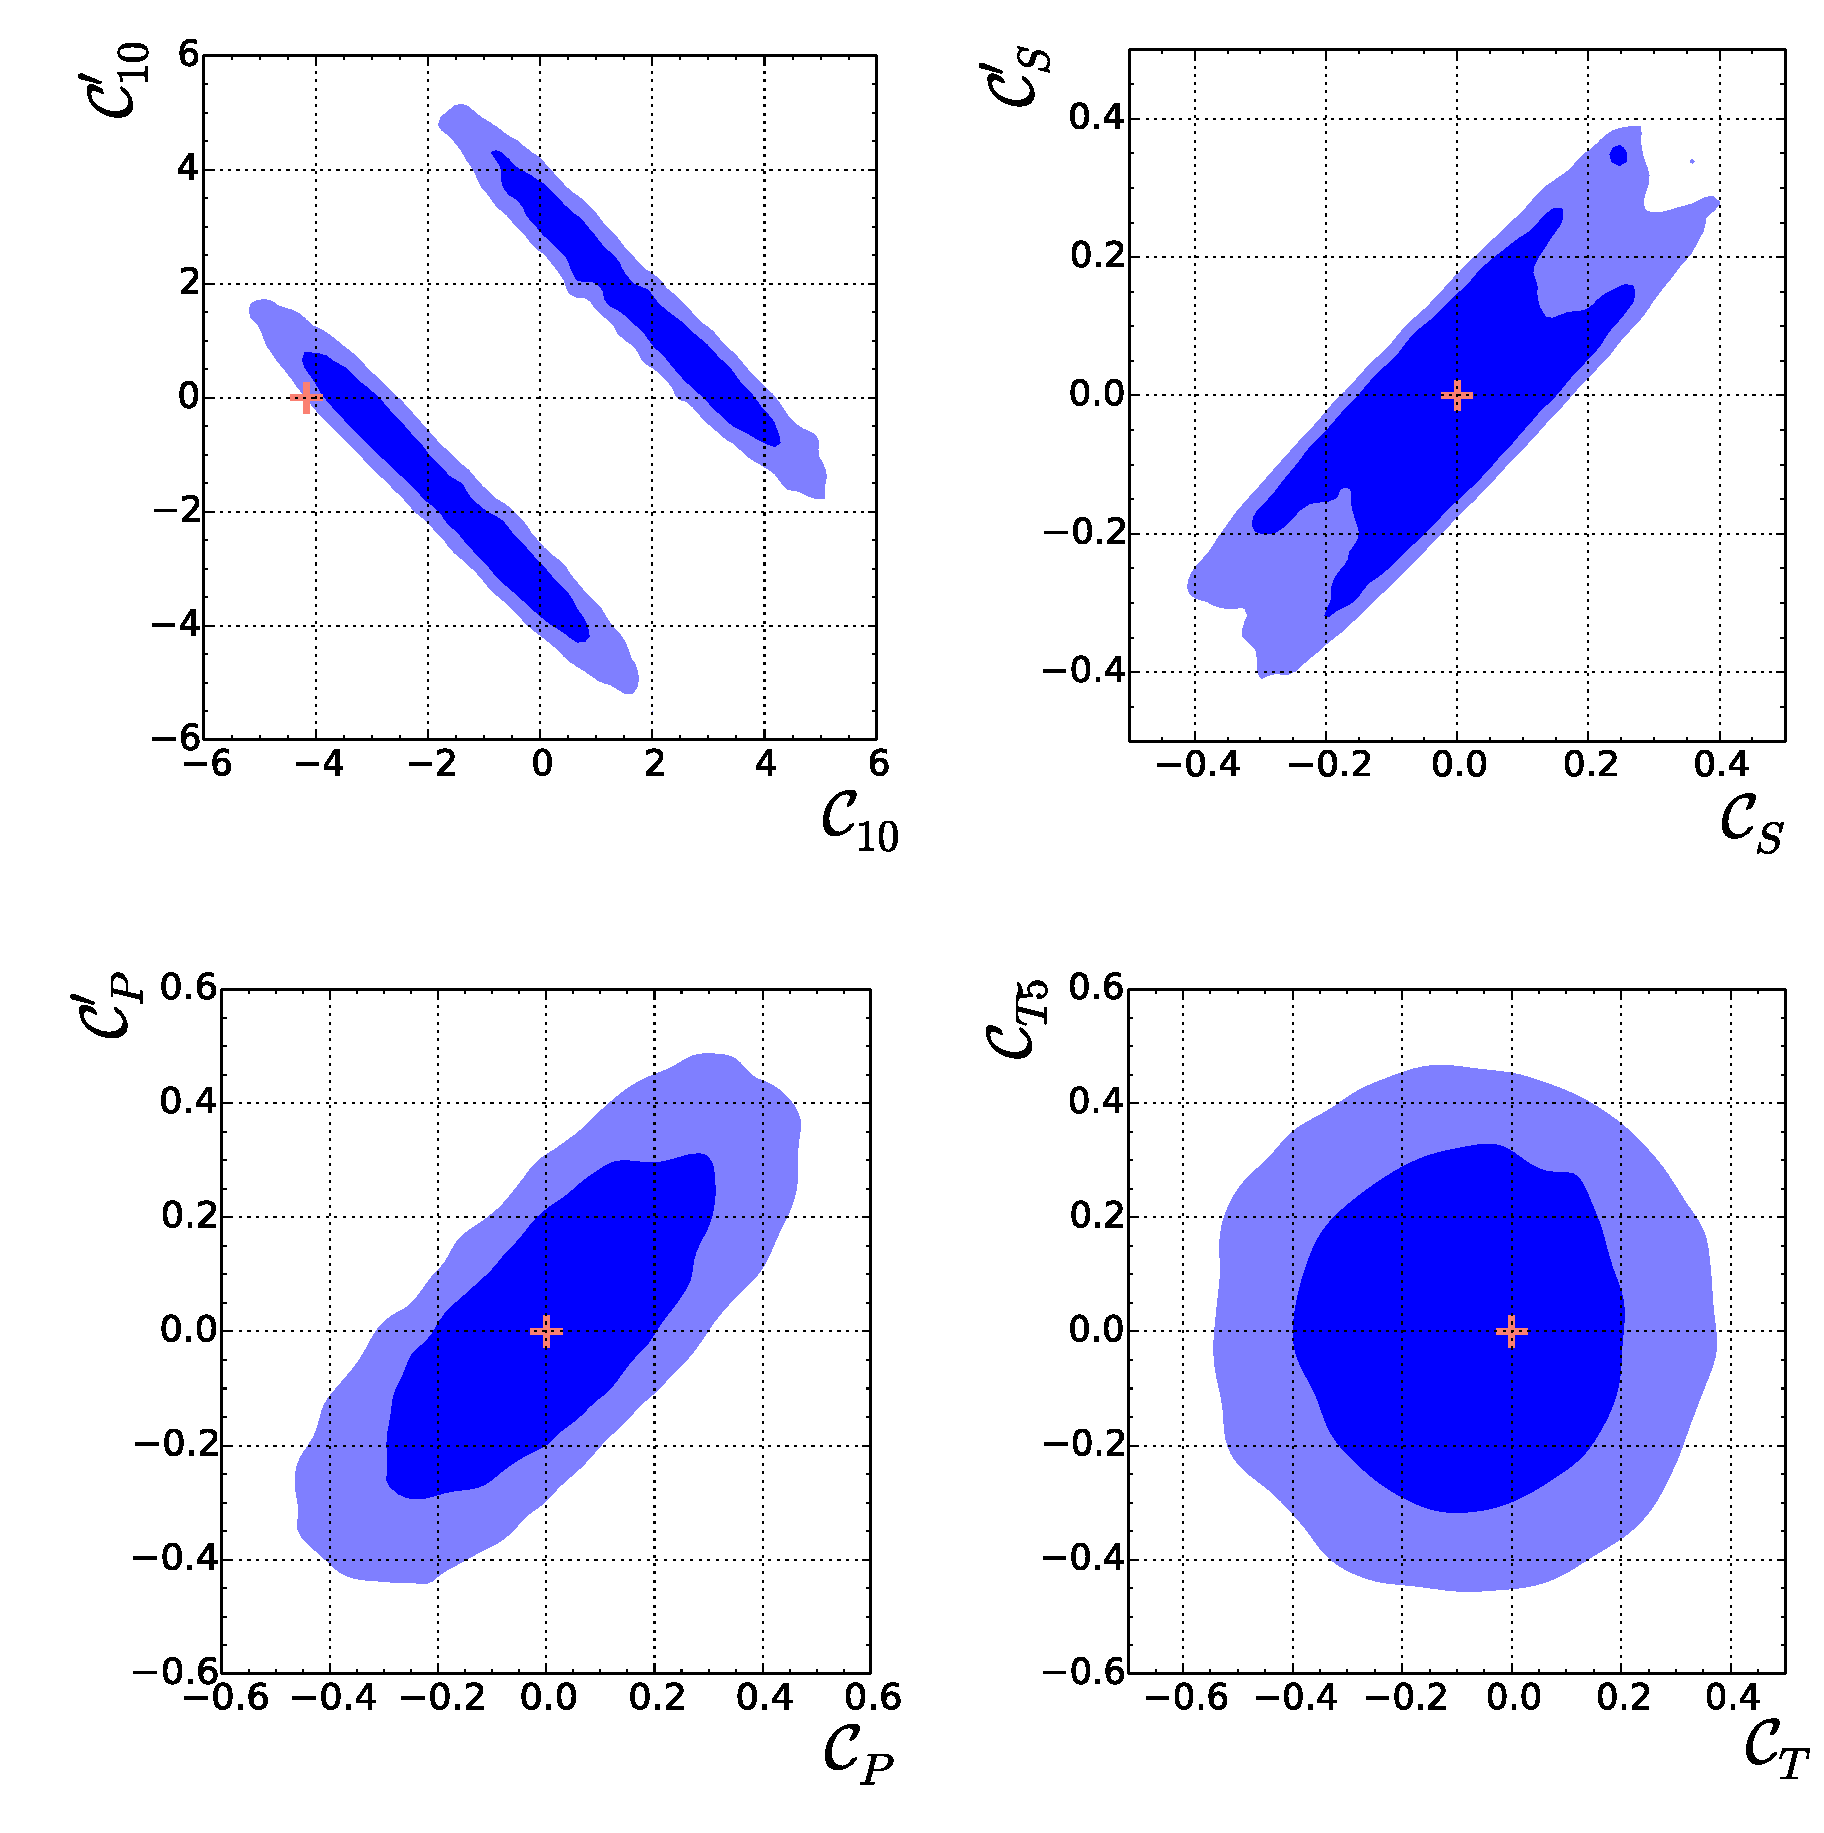
\includegraphics[width=\textwidth]{figures/Wilson_coeff_2d}

        \column{0.35\textwidth}
            \begin{itemize}
                \uncover<2->{\item first \emph{simultaneous} fit}
                \uncover<3->{\item interference $\mathcal{C}_{10} ^{(\prime)} \leftrightarrow \mathcal{C}_{S,P} ^{(\prime)}$
                        in $ \mathcal{B}(B_s\rightarrow \mu^+\mu^-) $
                            \begin{itemize}
                                \uncover<4->{\item[$\Rightarrow$] larger uncertainty than obtained for fixed $\mathcal{C}_{10} ^{(\prime)} = \mathcal{C}_{10} ^{(\prime) \mathrm{SM}}$ \newline {\tiny \href{http://arXiv.org/abs/1205.5811}{arXiv:1205.5811}, \href{http://arXiv.org/abs/1206.0273}{arXiv:1206.0273}, \href{http://arXiv.org/abs/1407.7044}{arXiv:1407.7044}}}
                            \end{itemize}
                      }
            \end{itemize}
            \vspace{6.5mm}

    \end{columns}

}

\subsection{Nuisance parameters}

\slide[t]{

    \begin{center}
        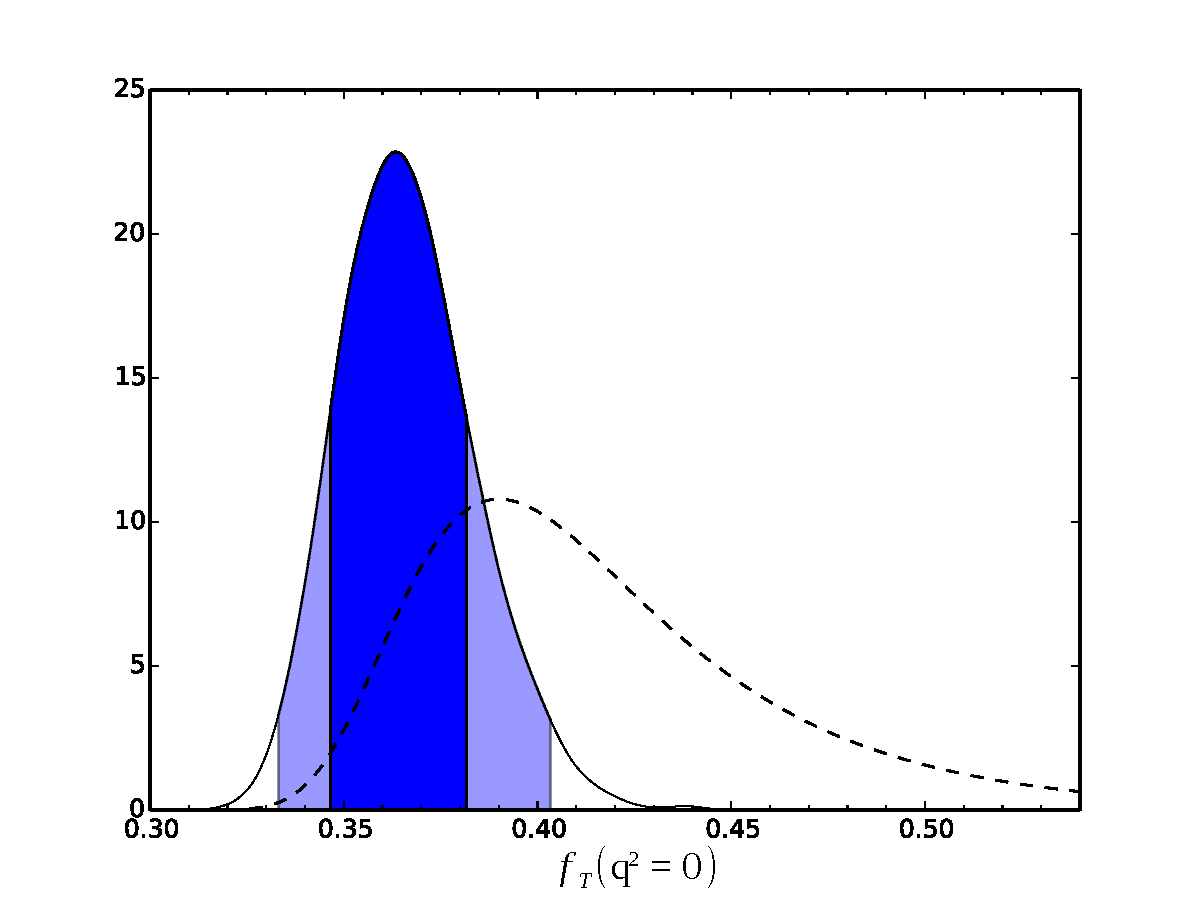
\includegraphics[width=0.9\textwidth]{figures/FF_ft0}
    \end{center}

}

\slide{

    \begin{center}
        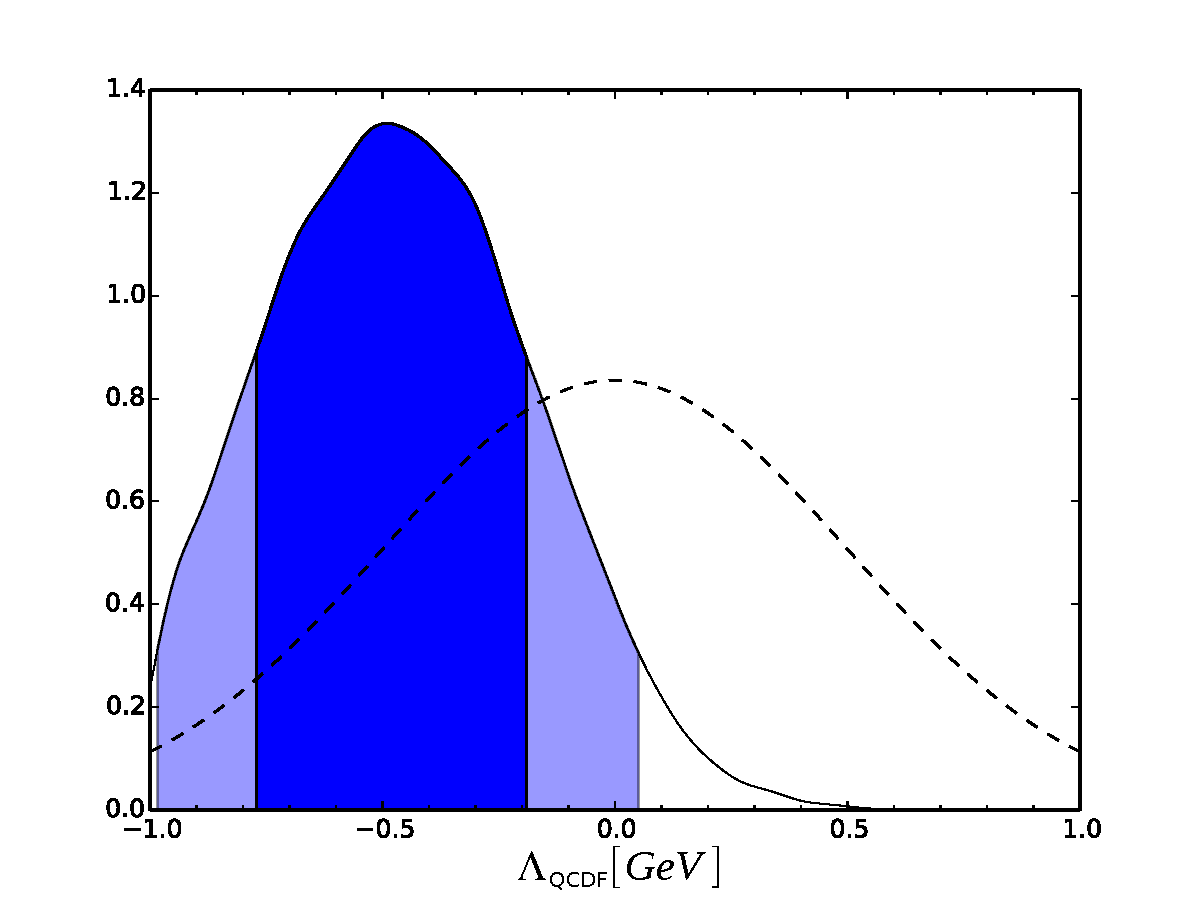
\includegraphics[width=0.9\textwidth]{figures/SL_large_recoil}
    \end{center}

}

\subsection{Sampling algorithm}

\slide[t]{

{\large\textbf{Difficulties}}

\begin{columns}[c] % The "c" option specifies centered vertical alignment while the "t" option is used for top vertical alignment

\column{.45\textwidth} % Left column and width

\begin{itemize}
    \uncover<2->{\item curse of dimensionality}
    \uncover<3->{\item multimodality}
    \uncover<4->{\item degeneracies}
\end{itemize}

\uncover<5->{\Huge \textcolor{red}{no standard algorithm so far}}

\column{.6\textwidth} % Right column and width


\begin{center}
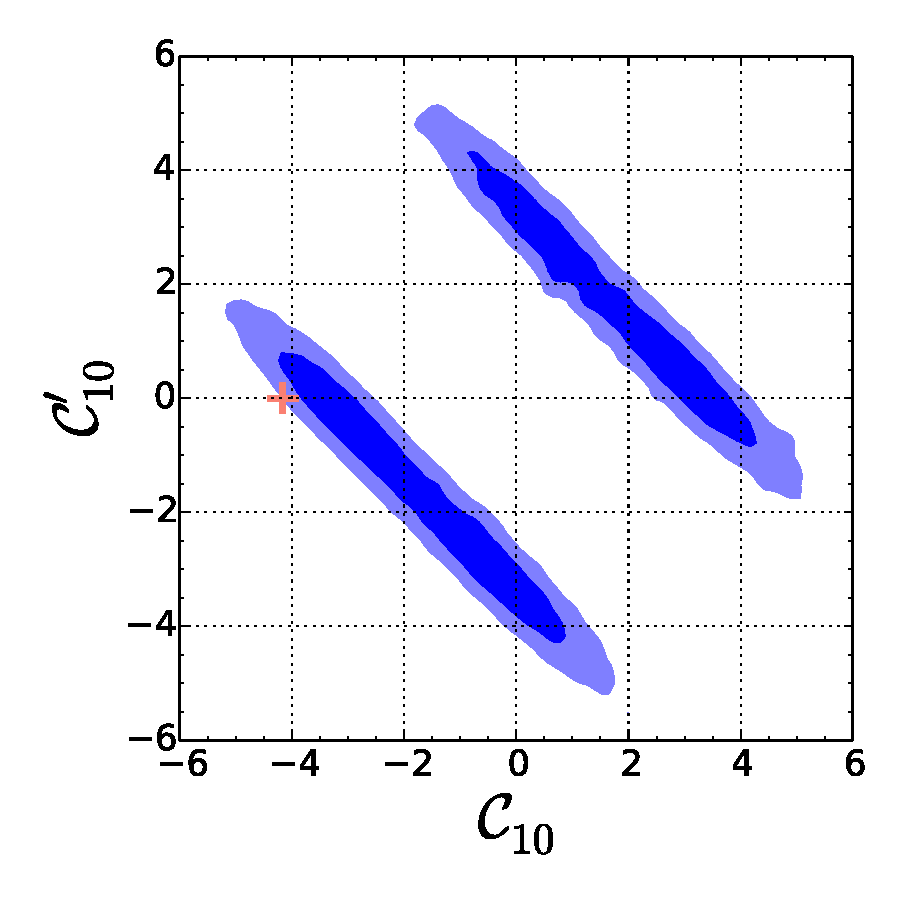
\includegraphics[height=0.7\textheight]{figures/C10_C10p}
\end{center}


\end{columns}

}

\slide{

    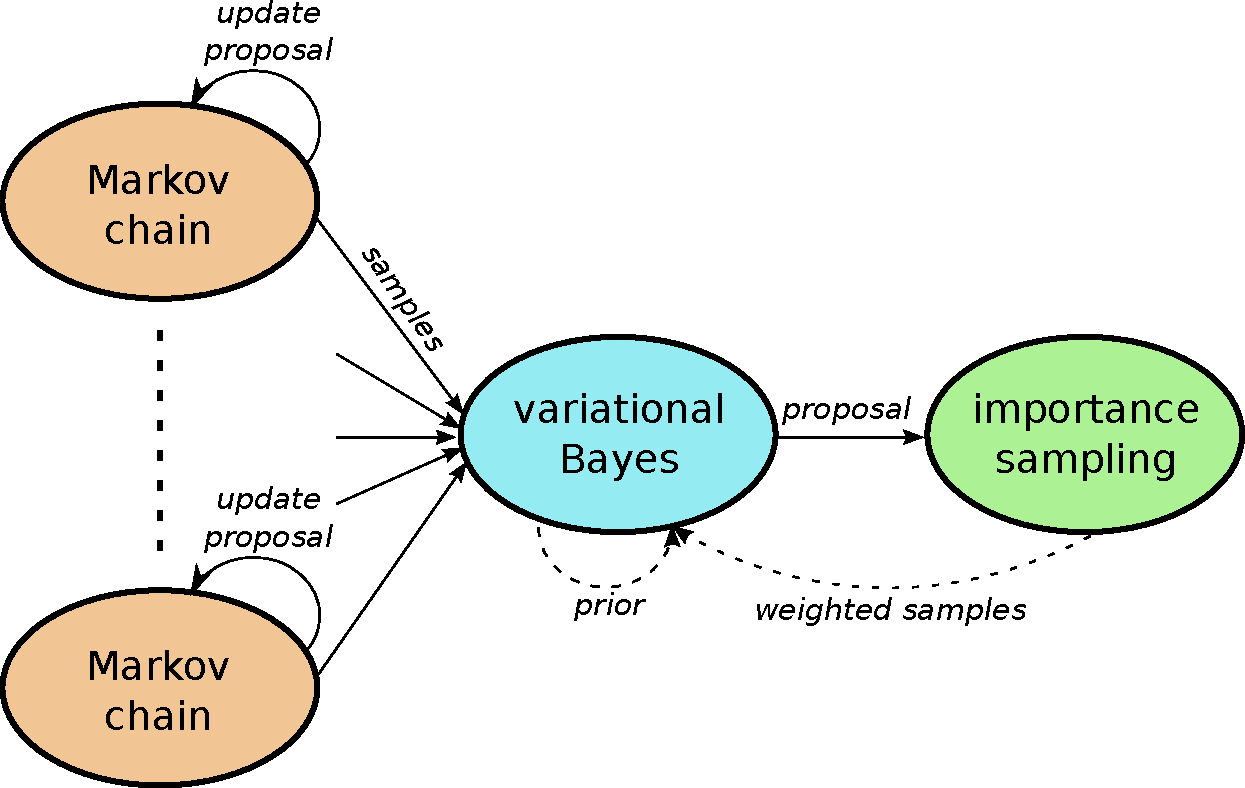
\includegraphics[width=\textwidth]{figures/algorithm}

    \begin{center}
        \url{https://pypi.python.org/pypi/pypmc}
    \end{center}

}

\subsection{Conclusion} %TODO: reconsider this

\slide[c]{

    \begin{itemize}
        \uncover<2->{\item model-independent search for new physics}
        \newline
        \uncover<3->{\item \red{simultaneous} fit {\footnotesize of $\mathcal{C}_S ^{(\prime)} , \mathcal{C}_P ^{(\prime)} , \mathcal{C}_T , \mathcal{C}_{T5} , \text{and} ~ \mathcal{C}_{10} ^{(\prime)}$}
            \begin{itemize} \item[$\Rightarrow$] updated, data-driven constraints \end{itemize} } \

        \uncover<4->{\item no significant deviation from the SM}
        \newline
        \uncover<5->{\item need better theoretical control {\footnotesize (form factors, subleading QCDF)}}
        \newline
        \uncover<6->{\item sampling algorithm {\footnotesize to handle multimodality in $\text{dim} = \mathcal{O}(40)$}}
    \end{itemize}

}

\subsection{Outlook}

\slide[c]{

    {\large \textbf{$\boldsymbol{B\rightarrow K^\ast \mu^+\mu^-}$ angular analysis} \newline }

    \begin{itemize}

        \uncover<2->{\item $J_{6c}$, $ (J_{1s} - 3J_{2s}) $, $ (J_{1c} - J_{2c}) $ %TODO: last observable "+" or "-" --> ask Christoph
              \newline $\red{\mathrm{SM}}$\red{-contributions suppressed} $\mathcal{O}\Big(\frac{m_\ell}{\sqrt{q^2}}\Big)$ }

        \uncover<3->{\item LHCb currently assumes $ \mathcal{C}_{S , P , T , T5} ^{(\prime)} = 0 \Rightarrow P (\mathcal{D} | \boldsymbol{O} , \red{\overset{ \text{\large \red{\thinspace{}\thinspace{}invalid} } }{\overbrace{\cancel{ \textcolor{red}{\boldsymbol{\theta} , \mathrm{M} } } }}} )$
              \newline {\tiny \url{http://www.physi.uni-heidelberg.de/Forschung/he/LHCb/documents/WorkshopNeckarzMar14/NeckarzimmernKstmumuExp.pdf} } \
              \newline}

        \uncover<4->{\item {\Large paper work in progress}}

    \end{itemize}

}

\end{document}
